% !TEX root = deckblatt4.tex
\section{Br\"uckengleichrichter}
\subsection{Aufgabenstellung}
In dieser Aufgabe musste ein Br\"uckengleichrichter aufgebaut werden und Zeit- und Frequenzmessungen durchgef\"uhrt werden. Des weiteren sollte eine Fourierreihe Berechnet und mit den Ergebnissen verglichen werden.

\subsection{Messschaltung}
\begin{figure}[ht!]
  \begin{center}
    \begin{circuitikz}\draw
    (0,0) to[sI] (0,6) to[Do] (7,6) to[R={$R_1$}{$=1M$}](7,0) to[Do] (0,0)
    (2,0) to[short, *-] (2,4) -- (2.5,4) to[Do] (4.5,4) -- (5,4) to[short,-*] (5,6)
    (5,0) to[short, *-] (5,2) -- (4.5,2) to[Do] (2.5,2) -- (1.5,2) to[short, -*] (1.5,6)
    (0,0) node[ground]{};
    \draw[-latex] (8.5,6) -- (7.3,6);
    \draw (9.6,6) node[] {Kanal 1};
    \draw[-latex] (8.5,0) -- (7.3,0);
    \draw (9.6,0) node[] {Kanal 2};
    \draw (3.5,7) node[] {1N4148};
    \end{circuitikz}
  \end{center}
  \caption{Messschaltung}\label{bsp4_circ}
\end{figure}
\noindent
In Abbildung \ref{bsp4_circ} ist der Br\"uckengleichrichter, welcher f\"ur die nachfolgenden Messungen verwendet wird, zu sehen. Der Geleichrichter besteht aus vier Dioden (1N4148). Die Ausgangsspannung am Widerstand $R_1$ kann nicht einfach abgegriffen werden, da sonst ein Teil der Schaltung \"uber die Masse des Oszilloskops kurzgeschlossen werden w\"urde. Aus diesem Grund wurde mit 2 Kan\"alen gemessen und die Masse der Tastk\"opfe wurde mit der Masse des Funktionsgenerators an einen Punkt geschalten. Anschlie\ss{}end musste die Differenz mit der "Math"-Funktion des Oszilloskops berrechnet werden.

\subsection{Messung im Zeitbereich}
\begin{figure}[H]
 \begin{center}
  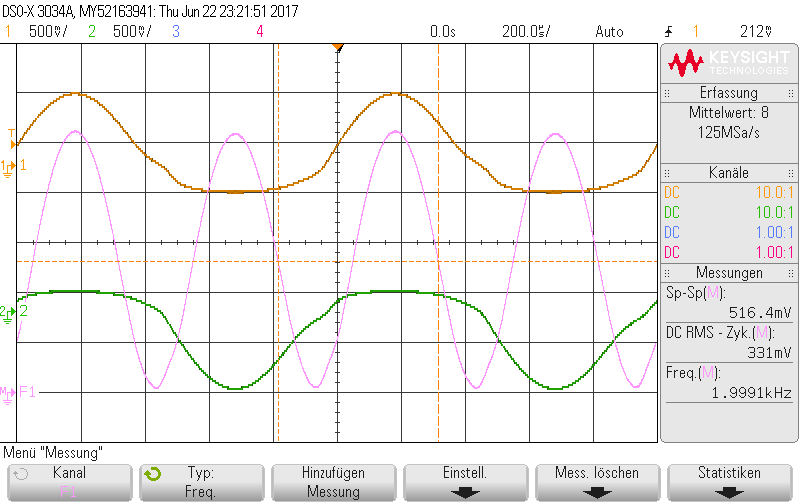
\includegraphics[height=6cm,width=12cm]{OsziBilder/bsp4_sin_time_2Vpp_UeUa.png}
 \end{center}
 \caption{Sinussingal $2V_{pp}$, $1kHz$}\label{bsp4_time2V}
\end{figure}
\noindent

\begin{figure}[H]
 \begin{center}
  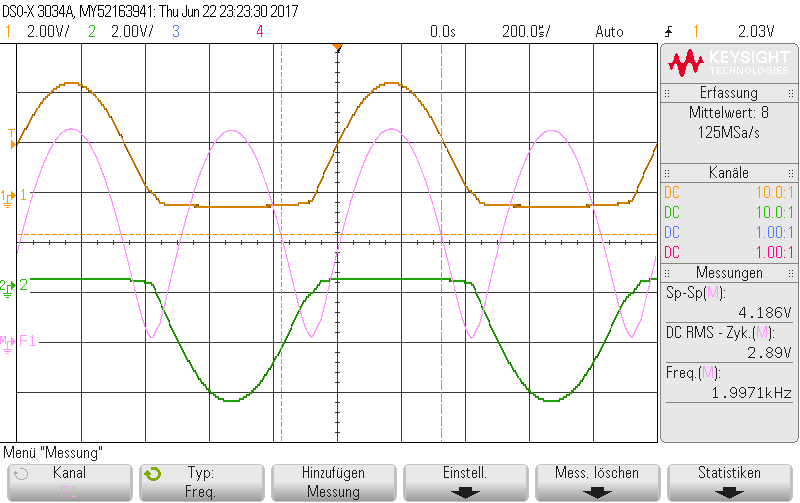
\includegraphics[height=6cm,width=12cm]{OsziBilder/bsp4_time_10Vpp_UeUa.png}
 \end{center}
 \caption{Sinussingal $10V_{pp}$, $1kHz$}\label{bsp4_time10V}
\end{figure}
\noindent
In den beiden Abbildungen \ref{bsp4_time2V} und \ref{bsp4_time10V} sind die Zeitsignale zu sehen. Die Differenz der beiden Kan\"ale ergibt den Gleichgerichteten Sinus, dieser hat die doppelte Frequenz als das Eingangssignal, jedoch den gleichen Effektivwert.

\subsection{Fouriereihe}
\begin{center}
  \begin{align*}
    |sin(t)| & \text{ ist eine gerade Funktion} \\
    S(f) &= \frac{a_0}{2} + \sum_{n=1}^{\infty} a_n * cos(nt) \\
    \text{Summensatz S8: } & 2sin(\alpha)cos(\beta) = sin(\alpha-\beta)+sin(\alpha+\beta) \\ \\
    a_0 &= \frac{1}{\pi}\int_0^{2\pi} |sin(t)| dt = \frac{2}{\pi}\int_0^{\pi} sin(t) dt = \frac{4}{\pi} \\ \\
    a_n &= \frac{2}{\pi}\int_0^{\pi} sin(t) * cos (nt) dt \\
    a_n &= \frac{1}{\pi}\int_0^{\pi} sin(t - nt) dt +  \frac{1}{\pi}\int_0^{\pi} sin(t + nt) dt\\
    a_n &= \frac{1}{\pi} \left[ \frac{cos(\pi(1-n))}{n-1} - \frac{cos(t(1+n))}{n+1} - \frac{1}{n-1} + \frac{1}{n+1} \right] \\
    a_n &= \frac{1}{\pi} \left[ -\frac{cos(\pi(1-n))}{n-1} + \frac{cos(t(1+n))}{n+1} - \frac{1}{n-1} + \frac{1}{n+1} \right] \\
    a_n &= \frac{1}{\pi} \left[ \frac{-(-1)^n (n+1) + (-1)^n (n-1) - (n+1) + (n-1)}{n^2-1} \right] \\
    a_n &= -\frac{1}{\pi} \left[ \frac{2(-1)^n + 1}{\pi(n^2-1)} \right] \\
    a_n &= \left\{\begin{array}{ll}
            0                     \hspace{2.5cm} \text{f\"ur n ungerade}\\
            \frac{4}{\pi(n^2-1)} \hspace{1.5cm} \text{f\"ur n gerade}
            \end{array}\right. \\
    |sin(\omega t)| &= \frac{2}{\pi} + \sum_{n=1}^{\infty}\frac{4}{\pi(n^2-1)} cos(2n\omega t)
  \end{align*}
\end{center}

\begin{figure}[H]
  \begin{center}
    \begin{tabular}{|c|c|} \hline
    $n$ & $V_{RMS}$ \\ \hline
    $0$ & $2,2508V$ \\ \hline
    $1$ & $1,5005V$ \\ \hline
    $2$ & $300,1mV$ \\ \hline
    $3$ & $128,6mV$ \\ \hline
    $4$ & $71,5mV$ \\ \hline
    $5$ & $45,5mV$ \\ \hline
    \end{tabular}
  \end{center}
  \caption{Berechneten Amplituden der f\"unf ersten Spektralanteile} \label{bsp4_SpecCalc}
\end{figure}



\subsection{FFT}
\begin{figure}[H]
 \begin{center}
  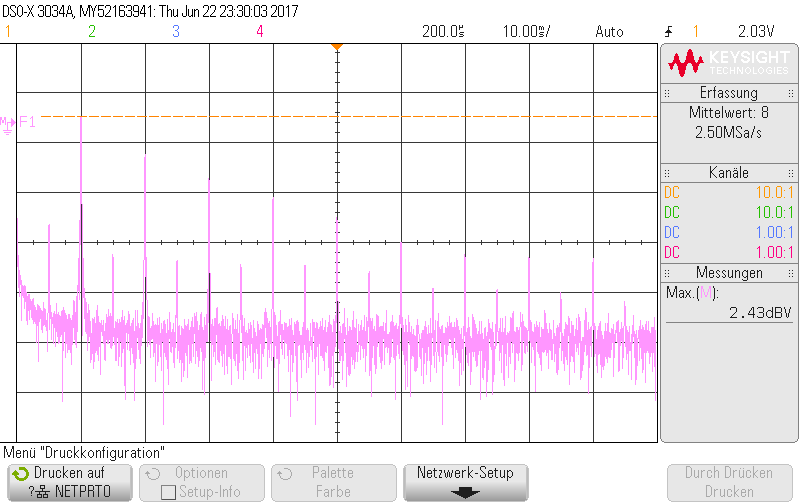
\includegraphics[height=6cm,width=12cm]{OsziBilder/bsp4_sin_fft_10Vpp_dB.png}
 \end{center}
 \caption{Sinussingal $10V_{pp}$, $10kHz$}\label{bsp4_fft}
\end{figure}
\noindent
Genau wie in den Berechnungen ist in der Messung zu erkennen, dass alle ungeraden Frquenzanteile quasi 0 ergeben (ca. $-30dB$) und die Amplituden mit steigender Frequenz rasch abnehmen.

\begin{figure}[H]
  \begin{center}
    \begin{tabular}{|c|c|c|} \hline
    $n$ & $V_{RMS}$ & Fehler[\%] \\ \hline
    $0$ & $2,083V$  & $8,1\%$   \\ \hline
    $1$ & $1,325V$    & $11,7\%$\\ \hline
    $2$ & $231,25mV$  & $22,9\%$\\ \hline
    $3$ & $75mV$      & $41,7\%$\\ \hline
    $4$ & $31,25mV$   & $56,3\%$\\ \hline
    $5$ & $12,2mV$    & $73,2\%$\\ \hline
    \end{tabular}
  \end{center}
  \caption{Messwerte der f\"unf gr\"o\ss{}ten Spektralen Komponenten} \label{bsp4_SpecMess}
\end{figure}
\noindent
In Tabelle \ref{bsp4_SpecMess} wurden die ersten f\"unf gro\ss{}en Spektralanteile mithilfe der Cursor Funktion gemessen und mit den in Tabelle \ref{bsp4_SpecCalc} berechneten Werten verglichen. Wie unschwer zu erkennen ist, ist bereits der Gleichanteil mit $8,1\%$ Fehler behaftet, der Fehler beim ersten Spektralanteil ist mit $11,7\%$ noch um etwas gr\"o\ss{}er. Dies ist unter anderem mit dem Spannunsabfall an den Dioden in der Gleichrichter Schaltung und etwaigen Messungenauigkeiten zu begr\"unden, auch die Amplitudengenauigkeit der Fensterfunktion spielt hier eine große Rolle. Diese Fehler wachsen mit steigender Frequnez sehr rasch, bei $5*f_g$ liegt dieser bereits bei $73,2\%$.
